% Written by Ayemane Bouarbi


Une grande étape de la réalisation de notre jeu vidéo passe par la création d'un style graphique dédié, complet et agréable à la vue.
Nous avons consacré un effort considérable à définir et à mettre en œuvre un style graphique cohérent qui non seulement correspond à la vision artistique du jeu, mais qui renforce également l'expérience immersive pour les joueurs.
\\

Cette phase de conception a également impliqué une collaboration entre les différents membres du groupe, notamment ici entre le directeur artistique (Ayemane Bouarbi et le responsable de l'intégration \textit{Godot}.


\subsubsection*{\hspace*{0.6cm}Style graphique}

Le choix du style graphique pixel art en 2D pour \gameName provient du choix réfléchi de l'esthétique du jeu et son potentiel à immerger les joueurs dans un monde magique et riche en aventure.
En effet, ce choix s'est révélé être une décision artistique judicieuse.
Ce style graphique simple et détaillé à la fois confère au jeu un charme unique tout en permettant une représentation qualitative des environnements et des personnages.
De plus, l'atmosphère visuelle du jeu est soigneusement choisie en fonction des différentes zones du jeu pour une meilleure immersion des joueurs dans l'univers apportée par \gameName.
\\

En plus d'évoquer la nostalgie des jeux classiques, le pixel art nous offre une flexibilité artistique tout en étant relativement léger en termes de ressources.
Inspiré par des jeux emblématiques tels que \textit{Stardew Valley}, \textit{Undertale}, ainsi que par autres pixel arts correspondant à l'ambiance recherchée en ligne.

\begin{figure}[H]
    \centering
    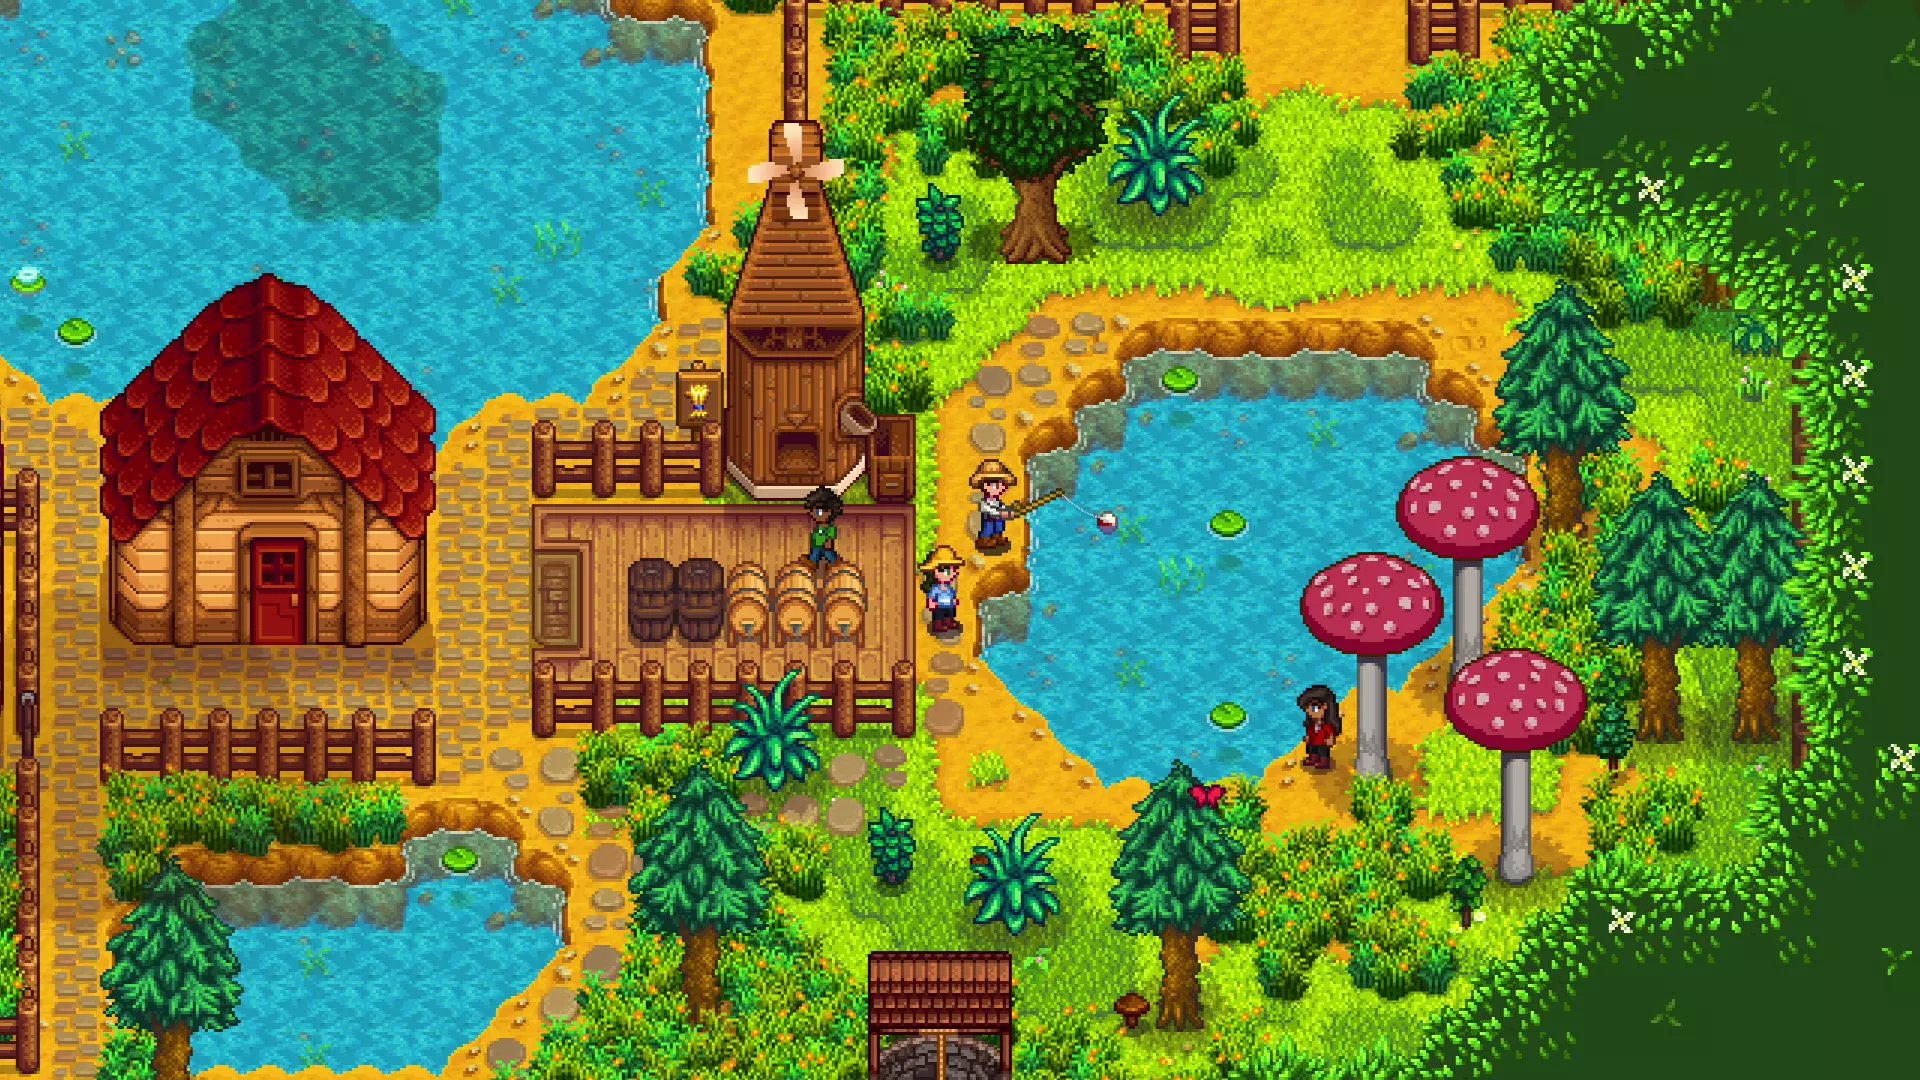
\includegraphics[width=0.8\textwidth]{2.game/assets/design1.png}
    \caption{Le jeu Stardew Valley}
    \label{fig:design1}
\end{figure}
\begin{figure}[H]
    \centering
    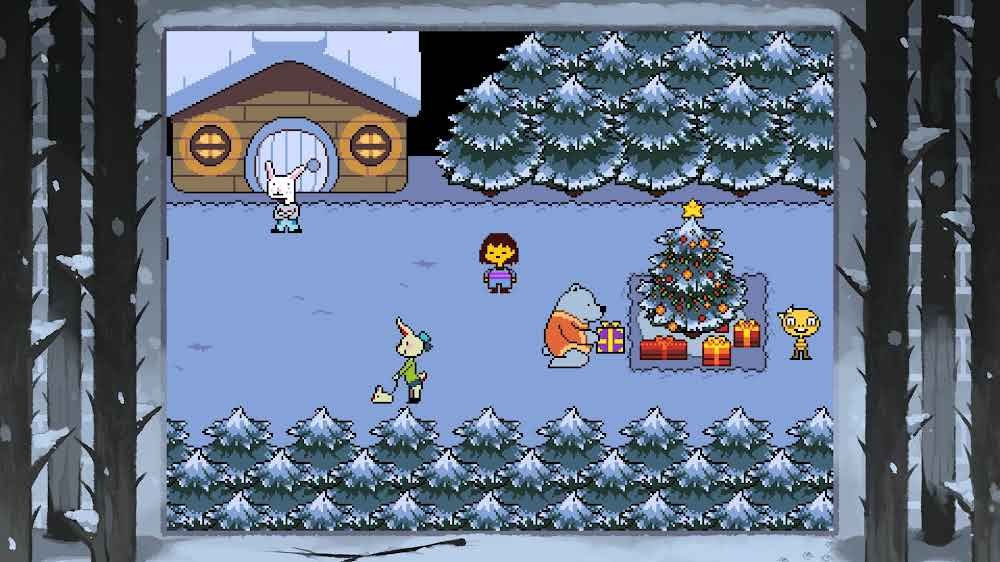
\includegraphics[width=0.8\textwidth]{2.game/assets/design2.png}
    \caption{Le jeu Undertale}
    \label{fig:design2}
\end{figure}

Ainsi le pixel art permet une expressivité artistique unique, offrant la possibilité de créer des environnements et des personnages riches en détails tout en conservant un charme visuel distinctif.
Les exemples concrets de textures créées pour le jeu (cf. \ref*{fig:design3}) illustrent le style en pixel art que nous avons développé.
En explorant le monde de \gameName, les joueurs seront immergés dans un univers visuellement époustouflant, où chaque pixel contribue à raconter une histoire captivante.


\subsubsection*{\hspace*{0.6cm}Création des textures}

La création des textures pour \gameName a été une entreprise passionnante et méticuleuse, réalisée principalement à l'aide d'outils de retouche d'image comme \textit{GIMP}.
Cette approche a permis à notre équipe de bénéficier d'une grande souplesse créative tout en exploitant les fonctionnalités pratiques de ce logiciel open-source.
\\

Le processus de création des textures commence par la conceptualisation, où nous explorons différentes idées et concepts pour chaque élément du jeu, qu'il s'agisse d'environnements, de personnages ou d'objets.
Une fois le concept finalisé et validé, nous passons à l'étape de la concrétisation, où le directeur artistique réalisera les textures.
Pour les réaliser, nous nous inspirons d'image ainsi que de texture d'autre jeu existant correspondant au style choisi, faisant ainsi office de modèle adapté à notre projet.
\\

L'intégration de détails et de textures nécessite souvent plusieurs itérations et ajustements pour parfaire le rendu final.
Nous accordons également de l'attention aux petits détails qui contribuent à enrichir l'expérience visuelle du joueur, qu'il s'agisse des textures de sol, la fluidité des animation des entités, ou encore la création de variantes de certaines textures afin de casser la monotonie du décor.

\begin{figure}[H]
    \centering
    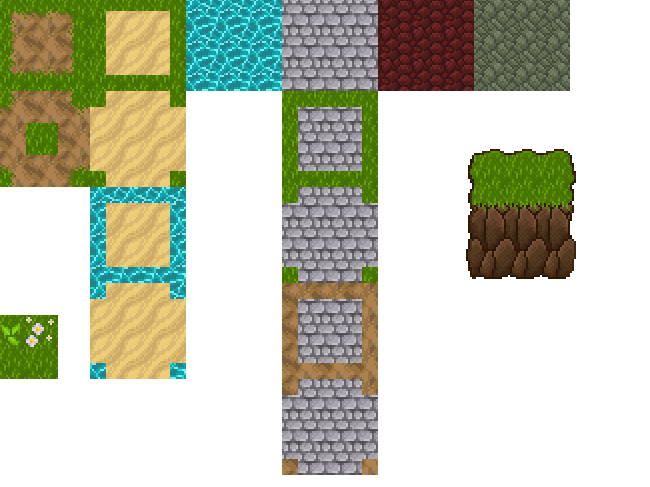
\includegraphics[width=0.8\textwidth]{2.game/assets/design3.png}
    \caption{Quelque exemples de texture en cours de création}
    \label{fig:design3}
\end{figure}

Chaque texture est ensuite implémentée et testée dans le jeu pour évaluer son apparence et son intégration dans l'environnement de jeu. Des ajustements supplémentaires sont apportés si nécessaire pour garantir une cohérence visuelle et une immersion optimale.
\\

En fin de compte, notre objectif est de créer des textures qui non seulement embellissent le monde de \gameName, mais qui racontent également une histoire et enrichissent l'expérience de jeu.
Grâce à notre engagement ainsi qu'à notre rigueur dans le processus de création, nous sommes convaincus que les textures que nous avons créées contribuent de manière significative au succès et à l'attrait de notre jeu.

\subsubsection*{\hspace*{0.6cm}Intégration des éléments graphiques dans le jeu}

L'intégration des textures et des éléments graphiques dans \gameName est une étape cruciale pour créer une expérience immersive et cohérente pour les joueurs.
Notre processus d'intégration vise à garantir que chaque texture s'intègre harmonieusement dans l'environnement de jeu, renforçant ainsi l'atmosphère et l'esthétique globale du monde virtuel.
\\

Lors de l'intégration des textures, nous nous assurons d'abord de respecter les spécifications techniques du jeu, en veillant à ce que les dimensions, les formats et les résolutions des textures correspondent aux exigences des développeurs.
Une fois cette étape technique achevée, nous procédons à l'incorporation des textures dans les différents éléments du jeu, tels que les décors, les personnages et les objets, afin de donner vie à la carte dans laquelle le joueur va explorer.
\\

La conception de la carte de \gameName a été un processus méticuleux et essentiel, visant à créer un monde cohérent et immersif pour les joueurs à explorer.
Tout d'abord, une planification initiale a été effectuée sur papier pour définir les principaux éléments de la carte, tels que les zones géographiques, les villes et les donjons.
\\

Cette étape a permis de définir la structure globale du monde du jeu.
Ensuite, les différentes zones géographiques ont été créées avec soin, en tenant compte de leur positionnement relatif et de leur connexion les unes aux autres.
Chaque zone, qu'il s'agisse de forêts, de montagnes, de plaines ou de marais, a été imaginée avec ses propres caractéristiques visuelles et thématiques pour offrir une variété d'environnements aux joueurs.
\\

Des points d'intérêt ont été ensuite dispersés à travers la carte pour encourager l'exploration et offrir des récompenses aux joueurs.
Cela inclut des villages, des temples, des grottes, des trésors cachés et d'autres éléments interactifs qui enrichissent l'expérience de jeu.
Par la suite, les routes et les chemins ont été définis pour relier les différentes zones entre elles, offrant aux joueurs des voies de passage pour naviguer dans le monde du jeu.
Des itinéraires principaux aux sentiers secrets, chaque chemin a été conçu pour offrir une expérience de voyage variée et engageante.
\\

Et c'est en suivant le plan détaillé de la carte que celle-ci est implémentée.
Enfin, une phase d'équilibrage et d'ajustements a été réalisée, où des tests ont été effectués pour évaluer l'équilibre du monde du jeu en termes de difficulté, de progression et d'accessibilité.
Des ajustements ont été apportés pour garantir une expérience équilibrée et satisfaisante pour les joueurs.
\\

En intégrant de manière réfléchie les textures et les éléments graphiques dans \gameName, nous sommes confiants que nous créons un monde visuellement captivant et immersif qui ravira les joueurs et les plongera dans une aventure épique.


\subsubsection*{\hspace*{0.6cm}Bilan des réalisations graphiques actuelles}

Dans le développement de \gameName, nous avons maintenu un bon rythme de progression dans la réalisation des graphismes et des textures en alignant nos efforts sur les objectifs initiaux. La majeure partie des textures essentielles du jeu a été réalisée depuis.
La communication et la coordination entre les membres du groupe ont été essentielles pour surmonter ces défis et maintenir la qualité du jeu.
\\

Cependant malgré ces progrès significatifs sur l'avancement du jeu, toutes les textures ne sont pas finies : En effet, notre objectif initial était de finaliser toutes les textures pour le 1er mars, mais le processus de création artistique a présenté des défis imprévus.
La création de textures de qualité demande du temps, plus que ce que l'on avait estimé.
\\

Mais il est important de noter que ce retard n'impacte pas le bon déroulement du développement du jeu, étant donné que les textures les plus importantes (celle nécessaire pour le développement immédiat du jeu) ont déjà été créées en priorité.
\\

De plus, la majorité des textures étant déjà créés (en plus du style recherché pour les textures qui a déjà été trouvé), la création du reste des textures ne se fera pas attendre longtemps.
\\

La gestion efficace du temps et des ressources est essentielle.
Ainsi, une planification minutieuse et une répartition claire des tâches permettront de surmonter ces obstacles.
Ainsi malgré les défis rencontrés, notre engagement envers la qualité et notre détermination à respecter nos objectifs demeurent intacts.


\subsubsection*{\hspace*{0.6cm}Perspectives et objectifs futurs}

Pour commencer, nous identifions les tâches restantes sur les textures du jeu, en mettant l'accent sur les éléments graphiques prioritaire qui nécessite des ajouts immédiats (comme par exemple le rendu d'une ).
Une fois les texturé à  qui nécessitent encore des ajustements ou des ajouts.
Cela peut inclure la création de nouvelles textures pour des environnements ou des objets spécifiques, ainsi que des améliorations visuelles pour renforcer l'immersion du joueur.
\\

Nous établissons également un planning pour la finalisation de ces éléments graphiques manquants, en tenant compte des contraintes de temps et des ressources disponibles.
Ce planning est élaboré de manière réaliste, en prenant en compte les leçons tirées des retards précédents et en allouant suffisamment de temps pour chaque étape du processus de développement.
\\

De plus, nous restons ouverts à des propositions d'améliorations ou d'ajustements à apporter au design existant, en nous basant sur les retours des testeurs et les observations de l'équipe de développement.
Ces ajustements visent à affiner et à perfectionner l'esthétique du jeu, en optimisant chaque élément graphique pour offrir une expérience visuelle exceptionnelle.
\\

En parallèle de cela nous continuerons à intégrer le reste de la carte en jeu en suivant le plan prévu à cet effet, permettant ainsi aux autres membres du groupe de travailler sur un projet se rapprochant de plus en plus du résultat final.
\\

En conclusion, en ce qui concerne la réalisation artistique du projet, il nous reste la finalisation des textures ainsi que celle de l'intégration de la carte du jeu.
Avec une approche collaborative et un travail organisé , nous sommes convaincus que nous atteindrons nos objectifs et mèneront le projet de \gameName à bien.
\\

